\documentclass{article}
\usepackage{graphicx}
\begin{document}
\textbf{Seyed Ahmad Mousavi Zadeh - 403522145}

\section{Git and GitHub}

\subsection{Repository Initialization and Commits}
\paragraph{To start a project:}
\begin{enumerate}
    \item Create a new repository on GitHub.
    \item Clone the repository using the following command:
    \begin{verbatim}
    git clone <URL>
    cd <repository-name>
    \end{verbatim}
    \item Add files and commit them:
    \begin{verbatim}
    git add .
    git commit -m "Initial commit"
    git push origin main
    \end{verbatim}
\end{enumerate}
\subsection{GitHub Actions for LaTeX Compilation}
To set up \textbf{GitHub Actions}, follow these steps:
\begin{enumerate}
    \item Create the folder \texttt{.github/workflows}.
    \item Create a file named \texttt{latex-build.yml}:
    \begin{verbatim}
    name: Build LaTeX Document
    on:
      push:
        tags:
          - '*'
    jobs:
      build:
        runs-on: ubuntu-latest
        steps:
          - name: Checkout repository
            uses: actions/checkout@v2
          - name: Setup LaTeX
            uses: xu-cheng/latex-action@v2
            with:
              root_file: main.tex
              compiler: pdflatex
    \end{verbatim}
\end{enumerate}
\section{Exploration Tasks}

\subsection{Vim Advanced Features}
Advanced Vim features:
\begin{itemize}
    \item \textbf{Macros:} Record commands with \texttt{q} and repeat them with \texttt{@}.
    \item \textbf{Plugins:} Use popular plugins like \texttt{vim-fugitive} and \texttt{NERDTree}.
    \item \textbf{Terminal mode:} Open a terminal with the command \texttt{:term}.
\end{itemize}
\subsection{Memory Profiling}
\subsubsection{Memory Leak}
A \textbf{Memory Leak} occurs when allocated memory is not freed, causing system performance degradation.

\subsubsection{Valgrind}
The tool \textbf{Valgrind} helps identify memory issues and resolve \textbf{Memory Leaks}.
\subsection{GNU/Linux Bash Scripting}
\subsubsection{fzf}
For interactive file searching:
\begin{verbatim}
fd -e pdf | fzf
\end{verbatim}

\subsubsection{Opening PDFs with Zathura}
To open selected PDF files:
\begin{verbatim}
zathura $(fd -e pdf | fzf)
\end{verbatim}
\begin{figure}[h!]
    \centering
    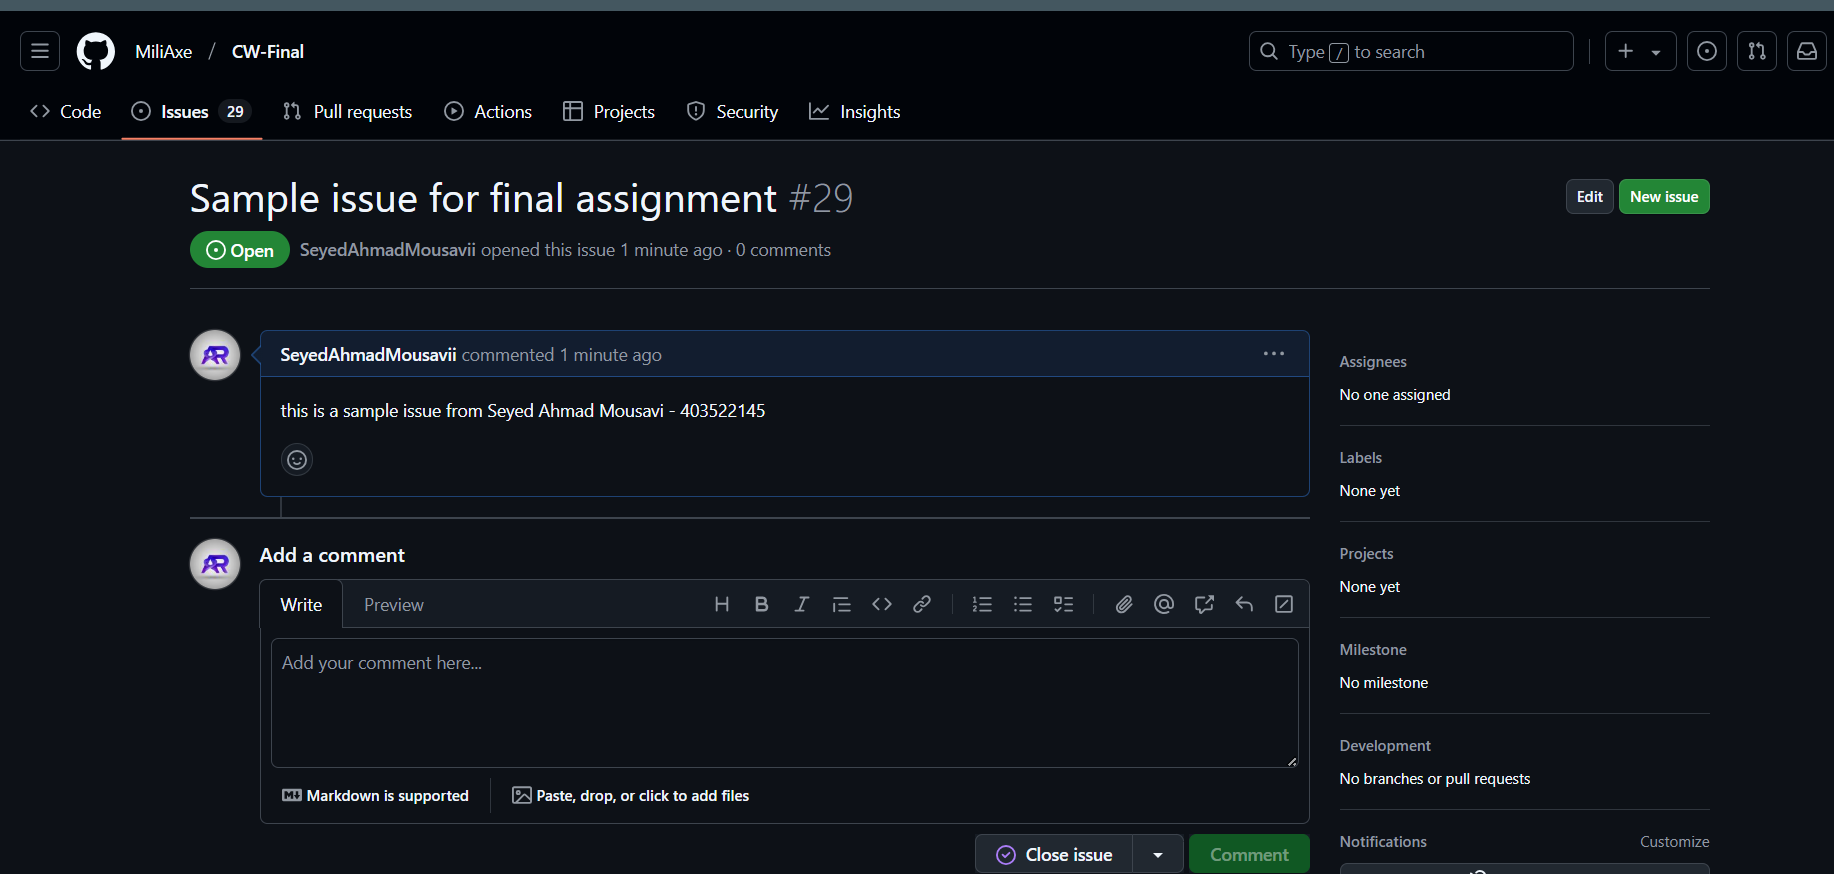
\includegraphics[width=0.5\textwidth]{assets/Screenshot 2025-01-15 233322.png}
    \caption{Sample Issue}
    \label{fig:example}
\end{figure}
\paragraph{Yes, I do see myself contributing to FOSS projects in the future. Open-source software plays a vital role in fostering innovation and collaboration, and I am excited about the idea of contributing to such projects. I would be particularly interested in contributing to development tools, such as text editors and automation scripts, as well as programming languages and scientific computing libraries. Additionally, I would like to contribute to improving documentation and tutorials for users, ensuring that open-source projects are more accessible to a wider audience. Overall, I believe that contributing to FOSS is a great way to learn, collaborate, and give back to the community.}
\paragraph{https://github.com/SeyedAhmadMousavii/Final-Assignment}

\end{document}
